% ======================================================================
% CHAPTER 3  RESULTS AND DISCUSSION
% ======================================================================
\chapter{Results and Discussion}
\label{ch:results}
This chapter follows the questions of Table~\ref{tab:experiments}. All figures and tables are regenerated by code from the committed result files, and every comparison is paired under common random numbers. Results that rest on assumed parameters are read as directions and rankings (Section~\ref{sec:params}).

\section{Calibrated Baseline}
\label{sec:res_base}
The calibrated base (coal, BOXN wagons, 292 rakes a year) gives a mean detention of \textbf{15.53 $\pm$ 0.33\,h} per rake, inside TERI's 14--17\,h band, while the physical chain alone (Layer 0, no paperwork) gives 4.05\,h. Of the rakes, 84\,\% exceed the 8\,h free time. Table~\ref{tab:attrib} shows who owns each hour of a rake's time at the siding: the terminal owns 73.5\,\%, the client 23.7\,\% and the Railway 2.9\,\%. Half of all rake time is spent queueing for the line, and the railway receipt and payment (client) take almost a quarter.

\begin{table}[!htbp]
\centering
\caption[Attribution of rake time by segment and owner, calibrated base]{Attribution of rake time by segment and owner, calibrated base (Layer 1, 50 rakes).}
\label{tab:attrib}
\small
\begin{tabular}{@{}llrr@{}}
\toprule
\textbf{Segment} & \textbf{Owner} & \textbf{Mean per rake (h)} & \textbf{Share} \\
\midrule
Queueing for the line & terminal & 35.45 & 51.0\,\% \\
Railway receipt and payment (M7) & client & 16.45 & 23.7\,\% \\
Release reporting (M5, M6) & terminal & 9.78 & 14.1\,\% \\
Loading & terminal & 4.14 & 6.0\,\% \\
Waiting for the crew & terminal & 1.69 & 2.4\,\% \\
Placement shunting & Railway & 1.01 & 1.5\,\% \\
Removal shunting & Railway & 0.97 & 1.4\,\% \\
\midrule
\multicolumn{2}{@{}l}{\textbf{Total by owner:} terminal 73.5\,\%, client 23.7\,\%, Railway 2.9\,\%} & & 100\,\% \\
\bottomrule
\end{tabular}
\end{table}

The client's share depends on the assumption that the railway receipt (M7) waits for railway office hours. The field data show electronic receipts for 99.7\,\% of coal, so in practice the client's share is smaller; this affects wagon time and attribution but not detention or demurrage, because M7 lies outside the billed window (Section~\ref{sec:res_break}).

\section{Where Detention Comes From}
\label{sec:res_where}
In a congested test case (one rake every 22\,h), the waiting split of Eq.~\eqref{eq:wsplit} gives:
\begin{itemize}
    \item \textbf{about 78\,\% administrative}: removing office hours alone removes 73.3\,\% of rake waiting, removing rework alone 10.9\,\%, and removing both 77.8\,\%;
    \item \textbf{at most 8\,\%} recoverable by optimal sequencing (the CP-SAT lower bound);
    \item \textbf{14\,\%} irreducible congestion, which no sequence can avoid.
\end{itemize}
Accordingly, no online dispatch rule beats first-come-first-served significantly at this operating point: SPT, the cost rule and Contract Net all give the same mean wait within their confidence intervals. Dispatch matters for \emph{fairness}, not for the mean: the cost rule without ageing lets the worst rake wait 161.2\,h, and Contract Net with ageing ($\alpha = 0.5$) cuts that to 108.1\,h ($-33$\,\%) at an unchanged mean wait. The lesson is that rakes wait mainly for offices and documents, not because they are served in the wrong order.

\section{Procedural versus Capital Interventions}
\label{sec:res_interv}
Figure~\ref{fig:interv} ranks the interventions against the campaign's own paired base (16.07\,h at the congested operating point of Section~\ref{sec:design}); opening every office round the clock gives the same detention as the terminal working round the clock and is not drawn separately. The three paperwork levers each save more than any capital lever. Digitalising the paperwork saves 8.98\,h per rake and cuts the share of rakes over free time from 86.8\,\% to 24.5\,\%; a second line with a second crew saves 0.58\,h, a factor of about 15.5. A second loading line \emph{alone} does not help (+0.28\,h, not significant), because with one crew two rakes compete for it, and a second shunting locomotive changes nothing, because shunting lies outside the billed window.

\begin{figure}[!htbp]
\centering
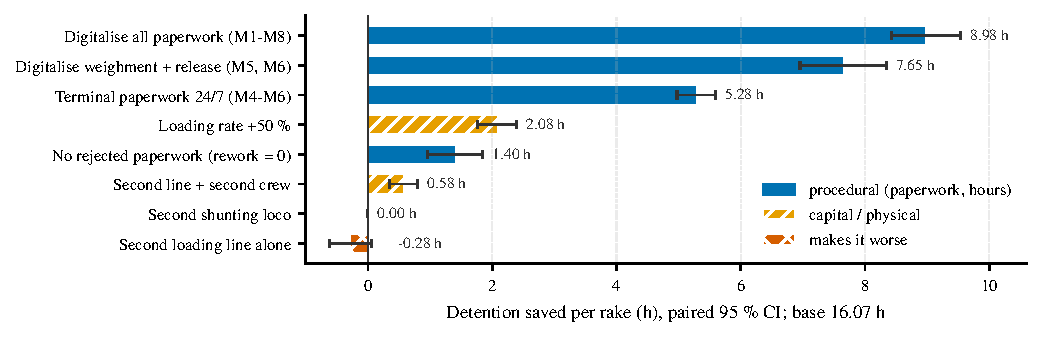
\includegraphics[width=0.94\textwidth]{figures/fig_interventions.pdf}
\caption[Detention saved per rake by each intervention]{Detention saved per rake by each intervention (Layer 4, 10 paired replications $\times$ 25 rakes, one rake every 22\,h). Procedural levers dominate; a second line without a crew does not help.}
\label{fig:interv}
\end{figure}

Detention, however, is only the billed window. A second line with a second crew barely shortens detention, but it cuts the \emph{wait before placement} from 44.3 to 17.2\,h, because two rakes can now be served at once. Procedural and capital levers therefore act on different things: procedure shortens each rake's stay on the line, while a second line adds a second place to stand. This difference becomes decisive for capacity (Section~\ref{sec:res_capacity}).

\section{Individual Effect of Every Factor}
\label{sec:res_sens}
Thirty-nine parameters and 27 conditions were varied one at a time over stated ranges (Figure~\ref{fig:sens}a). One calendar decision dominates: the number of hours a day the terminal's own paperwork (M4--M6) runs moves detention from 31.86\,h (8\,h a day) to 10.69\,h (24\,h a day), a swing of 21.2\,h, more than all physical parameters together. Release reporting (M6) and the loading rate follow, at 6.6\,h each. Each extra terminal hour helps less than the one before (Figure~\ref{fig:sens}b); extending today's 16\,h to 18\,h already yields 43\,\% of the round-the-clock gain (2.07 of 4.84\,h).

\begin{figure}[!htbp]
\centering
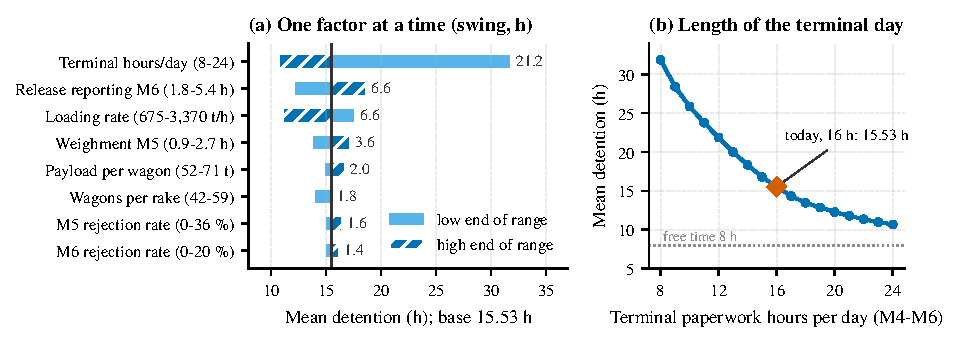
\includegraphics[width=0.94\textwidth]{figures/fig_sensitivity.pdf}
\caption[Individual effect of the top factors and of the length of the terminal day]{(a) Mean detention at the low and high end of each factor's range, top eight factors (number = swing in hours). (b) Detention for every length of the terminal paperwork day, with 95\,\% band (Layers 5 and 5b).}
\label{fig:sens}
\end{figure}

Morris screening (Figure~\ref{fig:morris}) confirms the same top three factors, terminal hours, M6 release time and the loading rate, followed by M5 weighment time. Their large $\sigma$ shows that their effects interact with other factors, which is why lever savings overlap (Section~\ref{sec:res_break}). All remaining parameters have $\mu^* < 2$\,h. Among the conditions, removing the release-reporting step entirely would save 6.55\,h, and two lines with two crews save only 0.67\,h of detention but 17.7\,h of waiting. Commercial parameters move money only: the penal multiplier raises demurrage per rake from Rs 75,962 to Rs 4.56 lakh at unchanged detention, so pricing cannot release a rake faster. With every factor at its favourable or unfavourable end, detention spans 3.54 to 51.41\,h.

\begin{figure}[!htbp]
\centering
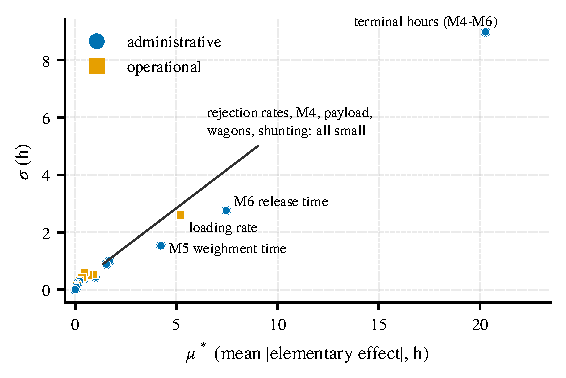
\includegraphics[width=0.62\textwidth]{figures/fig_morris.pdf}
\caption[Morris screening of the 39 parameters]{Morris screening of the 39 parameters ($R_M = 20$ trajectories, Eq.~\eqref{eq:morris}). Importance $\mu^*$ against interaction $\sigma$.}
\label{fig:morris}
\end{figure}

\section{Materials and Labour}
\label{sec:res_comm}
The ten commodity profiles of Table~\ref{tab:commodities} give base detentions from 13.4\,h (containers) to 22.0\,h (foodgrains); manual loading of bagged cargo makes loading itself long. Figure~\ref{fig:commodity} and Table~\ref{tab:levers} show how each lever acts on each material. Round-the-clock terminal paperwork and digital release help every material by a similar amount. Faster loading and digital weighment help all materials, by an amount that depends on the material. Silo loading and precise loading matter mainly for bulk, where overloading is frequent, and a second line with a crew changes sign across materials.

\begin{figure}[!htbp]
\centering
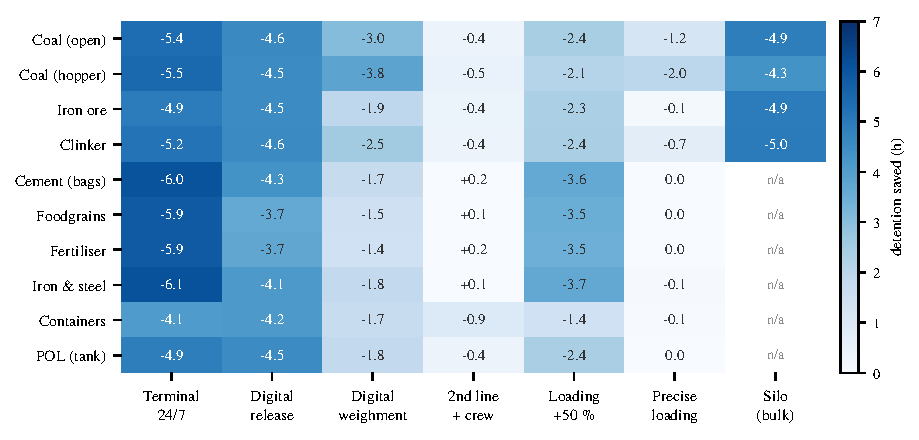
\includegraphics[width=0.94\textwidth]{figures/fig_commodity.pdf}
\caption[Change in detention per rake (h) for each lever and commodity]{Change in detention per rake (h) for each lever and commodity (Layer 6, paired against each commodity's own base). Silo loading applies only to mechanised bulk.}
\label{fig:commodity}
\end{figure}

\begin{table}[!htbp]
\centering
\caption[Change in detention per rake (h) across the ten commodity profiles, with the class of each lever]{Change in detention per rake (h) across the ten commodity profiles, with the class of each lever.}
\label{tab:levers}
\small
\begin{tabular}{@{}lcl@{}}
\toprule
\textbf{Lever} & \textbf{Range (h)} & \textbf{Class} \\
\midrule
Terminal paperwork 24/7 (M4--M6) & $-4.1$ to $-6.1$ & general, uniform \\
Digital release reporting (M6) & $-3.7$ to $-4.6$ & general, uniform \\
Loading rate $+50$\,\% & $-1.4$ to $-3.7$ & general, size depends on material \\
Digital weighment (M5) & $-1.4$ to $-3.8$ & general, size depends on material \\
Silo / rapid loading (bulk only) & $-4.3$ to $-5.0$ & material-specific \\
Precise loading (no overload) & $0.0$ to $-2.0$ & material-specific \\
Second line + second crew & $+0.2$ to $-0.9$ & material-specific (sign changes) \\
\bottomrule
\end{tabular}
\end{table}

\paragraph{Labour versus demurrage.} Loading 50\,\% faster can be bought with more labour. The labour break-even $B$ of Eq.~\eqref{eq:derived} is the most that can be spent per tonne before the extra labour costs more than the demurrage it avoids. It is about Rs 5.5 per tonne for mechanised bulk and Rs 9 per tonne for bagged cargo, i.e.\ about 46\,\% of the published coal handling rate and about 10\,\% of the bagged-cargo handling rate \cite{cwc}. Extra labour therefore pays for every material when it is paid per tonne. Paid per shift, it roughly breaks even for bulk and loses money for bagged cargo, because manual handling is already expensive per tonne.

\section{Breakdown of Time and Money}
\label{sec:res_break}
For the dominant real case, coal in open wagons at 292 rakes a year (register profile), four packages were simulated (Section~\ref{sec:design}): \emph{Today}; \emph{A}, terminal paperwork 24/7 plus digital release reporting, which needs no construction; \emph{B}, A plus precise loading; and \emph{C}, B plus 50\,\% faster loading.

\subsection{Where the Hours Come From}
Figure~\ref{fig:break}a splits the billed window exactly by cause (Eq.~\eqref{eq:dsplit}). Today, 6.5 of the 17.0\,h (38\,\%) are not productive work: 5.4\,h of waiting for an office to open and 1.1\,h of redoing rejected documents. Package A removes the office wait almost entirely; precise loading removes the remaining rework; faster loading then shortens the physical part. The bottleneck therefore \emph{moves}, from office hours to paperwork working time to loading speed, and each package attacks the next one.

\begin{figure}[!htbp]
\centering
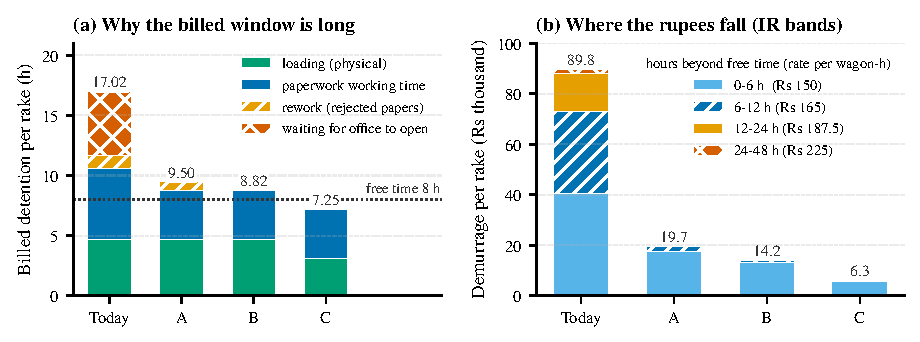
\includegraphics[width=0.94\textwidth]{figures/fig_breakdown.pdf}
\caption[Breakdown of billed detention and demurrage per package, coal siding]{Coal rake in open BOXN wagons, packages Today, A, B, C (Layer 8). (a) Billed detention split exactly by cause. (b) Demurrage per rake by IR charge band.}
\label{fig:break}
\end{figure}

\subsection{Where the Rupees Come From}
Money falls faster than time (Figure~\ref{fig:break}b and Table~\ref{tab:pack}), as the convexity of Eq.~\eqref{eq:dem} predicts. Package A cuts detention by 44\,\% but demurrage by 78\,\%, because every hour removed lies above the free time and the dearer bands empty first: under A the 6--12\,h band falls from Rs 32,262 to Rs 1,900 per rake and the 12--24\,h band from Rs 15,152.5 to Rs 209. Over a year of 292 rakes, package A avoids Rs 2.05 crore of demurrage, B Rs 2.21 crore and C Rs 2.44 crore.

\begin{table}[!htbp]
\centering
\caption[Outcomes per package, coal siding, 292 rakes a year]{Outcomes per package, coal siding, 292 rakes a year (Layer 8, means of 30 replications $\times$ 50 rakes). Wagons freed assume electronic railway receipts, as the field data show for coal.}
\label{tab:pack}
\small
\begin{tabular}{@{}lrrrr@{}}
\toprule
 & \textbf{Today} & \textbf{A} & \textbf{B} & \textbf{C} \\
\midrule
Detention per rake (h) $\downarrow$ & 17.02 & 9.50 & 8.82 & 7.25 \\
Rakes over free time (\%) $\downarrow$ & 90 & 67 & 59 & 28 \\
Wait before placement (h) $\downarrow$ & 37.4 & 20.2 & 19.4 & 17.9 \\
Line held per rake (h) $\downarrow$ & 19.0 & 11.5 & 10.8 & 9.2 \\
Demurrage per rake (Rs) $\downarrow$ & 89,786 & 19,651 & 14,195 & 6,265 \\
Demurrage avoided (Rs crore/yr) $\uparrow$ & -- & 2.05 & 2.21 & 2.44 \\
Overload and unused capacity (Rs crore/yr) $\uparrow$ & -- & -- & 4.20 & 4.20 \\
Wagons freed (Rs crore) $\uparrow$ & -- & 47.6 (21.0) & 50.5 (22.3) & 56.4 (24.9) \\
\bottomrule
\end{tabular}
\end{table}

Precise loading also removes the register-measured loss $\Theta$ (Eq.~\eqref{eq:derived}) of Rs 1.44 lakh per rake, Rs 4.20 crore a year. Most of it is paid-but-unused wagon capacity, i.e.\ about 159\,t more coal per rake for the same freight, so it is a capacity gain rather than cash.

\subsection{Fair Split between Levers}
The levers overlap: alone they would save 13.51\,h, together they save 9.77\,h. Table~\ref{tab:shapley} gives the Shapley split (Eq.~\eqref{eq:shapley}) of package C. Terminal hours and digital release together account for 71\,\% of the saving, and both need no construction.

\begin{table}[!htbp]
\centering
\caption[Saving of package C per rake: each lever alone and its Shapley share]{Saving of package C per rake: each lever alone and its Shapley share (Layer 8, $2^5$ factorial).}
\label{tab:shapley}
\small
\begin{tabular}{@{}lrrrr@{}}
\toprule
\textbf{Lever} & \textbf{Alone (h)} & \textbf{Shapley (h)} & \textbf{Share} & \textbf{Shapley (Rs per rake)} \\
\midrule
H Terminal paperwork 24/7 & 5.35 & 3.66 & 37\,\% & 33,613 \\
D Digital release reporting & 4.59 & 3.30 & 34\,\% & 28,265 \\
L Loading 50\,\% faster & 2.39 & 1.89 & 19\,\% & 13,955 \\
P Precise loading & 1.18 & 0.91 & 9\,\% & 7,689 \\
\midrule
\textbf{Total} & 13.51 & 9.77 & 100\,\% & 83,521 \\
\bottomrule
\end{tabular}
\end{table}

\subsection{Who Gains What}
The demurrage avoided by the client is income forgone by the Railway: it is a transfer, not a saving to the economy, and it is never added to the value of wagons. The Railway's gain is wagon time. Under package A each rake spends 24.6\,h less at the siding, which over a year returns 47.6 wagons to the fleet (Rs 21.0 crore at the price of a recent wagon order \cite{wagonvalue}). If the railway receipt waited for office hours, as the model assumes by default, the figure would be 37.5 wagons (Rs 16.5 crore); the data favour the larger figure. The terminal's gain is line capacity, measured next.

\section{Capacity of the Siding}
\label{sec:res_capacity}
The supervisor's final question was whether the siding can handle \emph{more rakes}. Layer 9 answers it by offering the coal siding more traffic, from 250 to 1,600 rakes a year, under each package and under two capital options (a second line with a second crew, alone and with package A), and recording the queue (Figure~\ref{fig:capacity}).

\begin{figure}[!htbp]
\centering
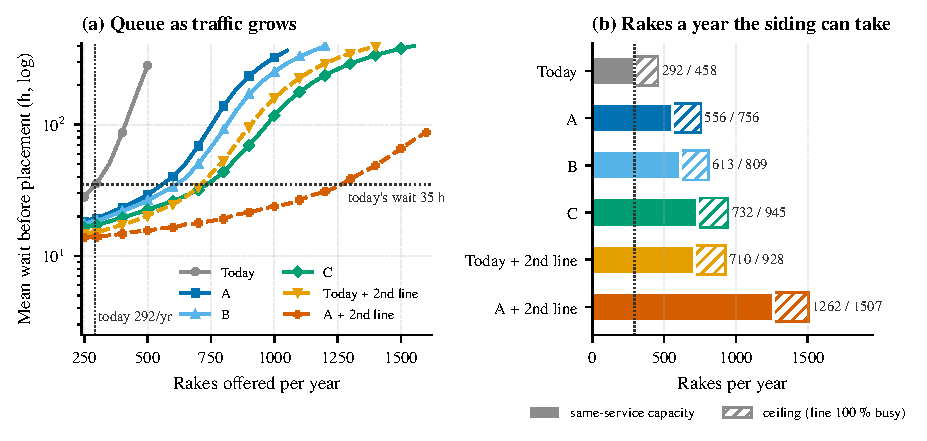
\includegraphics[width=0.94\textwidth]{figures/fig_capacity.pdf}
\caption[Queue and capacity of the coal siding as traffic grows]{Capacity of the coal siding (Layer 9, 30 replications $\times$ 200 rakes). (a) Mean wait before placement as the offered traffic grows; the dotted line is today's wait at 292 rakes a year. (b) Same-service capacity, Eq.~\eqref{eq:samesvc}, and capacity ceiling, Eq.~\eqref{eq:ceiling}.}
\label{fig:capacity}
\end{figure}

Today the siding works at 64\,\% line utilisation and rakes wait 35.0\,h before placement (the 200-rake runs of Layer 9 give 35.0\,h and a line hold of 19.1\,h, against 37.4\,h and 19.0\,h in the 50-rake runs of Table~\ref{tab:pack}; each comparison uses its own paired base). The queue grows steeply with traffic: at 400 rakes a year the wait passes 85\,h, and above the ceiling of 458 rakes a year the siding cannot clear what is offered (at 550 offered, only 448 a year are turned round). Table~\ref{tab:capacity} gives the capacity of each configuration.

\begin{table}[!htbp]
\centering
\caption[Capacity of the coal siding by configuration]{Capacity of the coal siding by configuration (Layer 9). Same-service capacity keeps the wait no longer than today's 35.0\,h.}
\label{tab:capacity}
\small
\begin{tabular}{@{}lrrrrr@{}}
\toprule
\textbf{Configuration} & \textbf{Line held} & \textbf{Ceiling} & \textbf{Same-} & \multicolumn{2}{c}{\textbf{Extra rakes vs today}} \\
\cmidrule(l){5-6}
 & \textbf{(h/rake)} & \textbf{(rakes/yr)} & \textbf{service} & \textbf{rakes/yr} & \textbf{\%} \\
\midrule
Today & 19.1 & 458 & 292 & -- & -- \\
A: paperwork 24/7, digital release & 11.6 & 756 & 556 & +264 & +90 \\
B: A + precise loading & 10.8 & 809 & 613 & +321 & +110 \\
C: B + faster loading & 9.3 & 945 & 732 & +440 & +151 \\
\midrule
Today + second line + second crew & 18.9 & 928 & 710 & +418 & +143 \\
A + second line + second crew & 11.6 & 1,507 & 1,262 & +970 & +332 \\
\bottomrule
\end{tabular}
\end{table}

Four findings follow.
\begin{enumerate}
    \item \textbf{Procedure nearly doubles capacity without construction.} Package A shortens the line hold from 19.1 to 11.6\,h, which raises the ceiling by 65\,\% (458 to 756 rakes a year) and lets the same line take 556 rakes a year at today's wait instead of 292 (+90\,\%). Package C, still without a new line, takes 732 (+151\,\%).
    \item \textbf{For capacity, a second line does matter.} Unlike detention, where a second line saved only 0.58\,h, capacity grows with the number of places to stand: a second line with a crew lifts same-service capacity to 710 rakes a year (+143\,\%), about the same as package C. The two kinds of lever are complements: procedure shortens each rake's stay, a line adds parallel service.
    \item \textbf{Combined, they multiply.} Package A with a second line and crew takes 1,262 rakes a year at today's wait, 4.3 times today's traffic, because each of two lines is also held for a shorter time.
    \item \textbf{More traffic does not raise detention or demurrage per rake.} Detention stays at about 17.0--17.5\,h (today) and 9.6\,h (A) at every traffic level, because it is set by paperwork, not by the queue. Under package A the siding could handle 550 rakes a year with a total demurrage bill of Rs 1.12 crore, against Rs 2.66 crore for 292 rakes today.
\end{enumerate}

\paragraph{What saturates first.} The line is the bottleneck in every configuration. At today's traffic the line is busy 64\,\% of the time, the loading crew 16\,\% and the shunting locomotive 7\,\%. Even at the same-service capacity of each configuration, the crew stays below 34\,\% and the locomotive below 29\,\% utilisation, so neither a second crew alone nor a second locomotive would add capacity until the line constraint is removed. The scaling question ``if traffic grows, what else must grow?'' therefore has a clear order: first shorten the line hold (procedure), then add a line with its crew; the locomotive and the crew follow much later.

\paragraph{Check against queueing theory.} The simulated queue was compared with the Pollaczek--Khinchine formula (Eq.~\eqref{eq:pk}) using the simulated line holds (Table~\ref{tab:pk}). With every office open, so that rakes reach the queue as a Poisson stream, the simulation agrees with the formula to within 0.91--1.03 times below 80\,\% line utilisation. With offices as modelled, the simulated queue is 1.04--1.96 times the formula below 80\,\% utilisation, highest for the packages with short line holds. The reason is mechanical: the forwarding note (M3) is cleared only in office hours, so rakes join the queue in bunches when the office opens, and bunched arrivals wait longer than Poisson ones. The check therefore confirms the queue mechanics and shows that office hours hurt twice: they lengthen each rake's stay and they bunch the arrivals.

\begin{table}[!htbp]
\centering
\caption[Simulated wait in the line queue against the Pollaczek--Khinchine formula]{Simulated wait in the line queue against the Pollaczek--Khinchine formula (Layer 9).}
\label{tab:pk}
\small
\begin{tabular}{@{}llrrrr@{}}
\toprule
\textbf{Configuration} & \textbf{Offices} & \textbf{Rakes/yr} & \textbf{Line use} & \textbf{Simulated (h)} & \textbf{Sim. / formula} \\
\midrule
Today & all open & 292 & 0.46 & 6.47 & 1.03 \\
Today & all open & 450 & 0.71 & 17.06 & 0.96 \\
A & all open & 292 & 0.39 & 3.90 & 1.01 \\
A & all open & 600 & 0.79 & 21.29 & 0.91 \\
\midrule
Today & as modelled & 292 & 0.64 & 21.96 & 1.15 \\
A & as modelled & 292 & 0.39 & 6.48 & 1.67 \\
C & as modelled & 292 & 0.31 & 4.31 & 1.96 \\
\bottomrule
\end{tabular}
\end{table}

The capacity figures rest on the same assumed paperwork times as the rest of the model, so they are read as directions and orders of magnitude: procedure roughly doubles the rakes a line can take, and procedure plus a second line roughly quadruples them.

\section{Wagon Damage and the Locomotive}
\label{sec:res_damage}
No published rate of wagon damage at loading sidings exists, so damage is an optional, assumed scenario (Section~\ref{sec:form}), following IR examination practice and audit findings \cite{irimee, cag}. Table~\ref{tab:dmg} compares the two rules for unfit wagons. Detaching the bad wagons adds a little detention, because the work falls inside the billed window. Returning the whole rake hardly changes the client's detention, because the rejected visit happens before the clock starts, but it costs the Railway about 2.3--2.6 times the wagon time of detaching. Detaching at the siding is the better rule for the system. The module measures time only; no repair price per wagon was available, so damage is not converted into rupees beyond its effect on demurrage.

\begin{table}[!htbp]
\centering
\caption[Extra hours per rake caused by defective wagons, coal siding today]{Extra hours per rake caused by defective wagons, coal siding today (Layer 8, assumed rates).}
\label{tab:dmg}
\small
\begin{tabular}{@{}lcccc@{}}
\toprule
 & \multicolumn{2}{c}{\textbf{Detach bad wagons}} & \multicolumn{2}{c}{\textbf{Return whole rake}} \\
\cmidrule(lr){2-3}\cmidrule(l){4-5}
\textbf{Defective wagons} & detention & arrival$\to$departure & detention & arrival$\to$departure \\
\midrule
0.5\,\% & +0.11 & +0.47 & +0.09 & +1.23 \\
1\,\% & +0.28 & +1.13 & +0.17 & +2.99 \\
2\,\% & +0.58 & +2.57 & +0.41 & +5.99 \\
\bottomrule
\end{tabular}
\end{table}

The shunting locomotive is modelled as a shared resource for placement, removal and detaching. A second locomotive saves no detention (Figure~\ref{fig:interv}) and the locomotive is busy at most 29\,\% of the time even at the highest same-service capacity (Section~\ref{sec:res_capacity}), so it is not a constraint in the modelled range. Locomotive breakdowns, late locomotives and the availability of train engines for the loaded haul are not modelled.

\section{Sufficiency of the Variable Set}
\label{sec:res_suff}
Layer 7 added each omitted factor of Table~\ref{tab:factors} at a realistic size, applied after the intervention so that no intervention can remove it, and re-ranked the six main interventions (Table~\ref{tab:suff}). The omitted factors change the \emph{level} of detention, from 15.5 to 23.1\,h with all of them together, but not the \emph{conclusions}: the ranking of the interventions is identical in all eight stress tests (Kendall $\tau = 1.00$), the best procedural lever saves 3.6--6.6 times as much as the best capital lever, and a second line without a crew never helps. The variable set is therefore sufficient for ranking interventions, the purpose of this study, though not for predicting absolute hours at a named siding.

\begin{table}[!htbp]
\centering
\caption[Omitted-factor stress test]{Omitted-factor stress test (Layer 7, 30 paired replications). Procedure / capital is the saving of the best procedural lever (digitalise all paperwork) divided by that of the best capital lever (faster loading).}
\label{tab:suff}
\small
\begin{tabular}{@{}lrcc@{}}
\toprule
\textbf{Omitted factor added} & \textbf{Base (h)} & \textbf{Kendall $\tau$} & \textbf{Proc./capital} \\
\midrule
None (model as built) & 15.53 & 1.00 & 4.4 \\
+1\,h physical delay inside free time & 17.00 & 1.00 & 4.8 \\
+3\,h physical delay inside free time & 19.99 & 1.00 & 5.3 \\
+1\,h unmodelled paperwork & 17.24 & 1.00 & 4.7 \\
+3\,h unmodelled paperwork & 20.68 & 1.00 & 5.4 \\
+50\,\% traffic & 15.87 & 1.00 & 4.7 \\
Loading disruptions (rate $-20$\,\%, sd $\times 2$) & 18.49 & 1.00 & 3.6 \\
Error rates $\times 2$ & 17.39 & 1.00 & 5.2 \\
All together & 23.07 & 1.00 & 6.6 \\
\bottomrule
\end{tabular}
\end{table}

\section{Summary: Time, Cost and Capacity}
\label{sec:res_summary}
Table~\ref{tab:summary} brings the three outcomes together for the coal siding. Package A, which needs no construction, nearly halves detention, cuts demurrage by more than three quarters, returns about 48 wagons to the fleet and nearly doubles the rakes the siding can take. Capital adds capacity but not speed; procedure adds both.

\begin{table}[!htbp]
\centering
\caption[Time, cost and capacity of the coal siding by package]{Time, cost and capacity of the coal siding by package (Layers 8 and 9).}
\label{tab:summary}
\small
\begin{tabular}{@{}lrrrr@{}}
\toprule
\textbf{Package} & \textbf{Detention (h)} & \textbf{Demurrage avoided} & \textbf{Wagons freed} & \textbf{Rakes/yr at today's wait} \\
 & & \textbf{(Rs crore/yr)} & & \\
\midrule
Today & 17.02 & -- & -- & 292 \\
A & 9.50 & 2.05 & 47.6 & 556 \\
B & 8.82 & 2.21 & 50.5 & 613 \\
C & 7.25 & 2.44 & 56.4 & 732 \\
\bottomrule
\end{tabular}
\end{table}
